%%%%%%%%%%%%%%%%%%%%%%%%%%%%%%%%%%%%%%%%%
%% Appendix section
Data analysis with the \textit{Tidyverse} \citep{tidyverse} package, for the R language \citep{R2023}, made the empirical analysis for this paper possible.

\subsection{UK Biobank Dataset Construction}

\subsubsection{Identifying Family Clusters by Genetic Similarity}
\label{appendix:identifying-families}

The UKB does not directly identify participants' family members, so I define family links using the genetic relatedness data.
I follow the approach in \citet{muslimova2025environment}, classifying genetically related pairs using the kinship coefficient and the identity-by-state zero coefficient (IBS$_0$).
These thresholds come from the KING relationship-inference procedure used to construct the UKB kinship matrix, which identifies genetically related pairs up to third-degree relatives \citep{manichaikul2010robust}.
The kinship coefficient measures the degree of genetic relatedness between two individuals, while IBS$_0$ measures the fraction of genotyped markers for which the two individuals share no alleles.
These two measures jointly distinguish different forms of close genetic relatedness.

\begin{table}[!h]
    \singlespacing
    \centering
    \small
    \caption{Genetically Identified Family Links in the UKB.}
    \begin{tabular}{l c c c}
        \\[-1.8ex]\hline \hline \\[-1.8ex] 
        Genetic link & Kinship Coefficient & IBS$_0$ & Count \\
        \\[-1.8ex]\hline \hline \\[-1.8ex] 
        % latex table generated in R 4.6.0 by xtable 1.8-8 package
% Mon May 18 14:34:51 2026
 Duplicate / Monozygotic twins & $> 0.3540$ &  & 179 \\ 
  1st degree / Parent-child & $0.1770$--$0.3540$ & $< 0.0012$ & 6,249 \\ 
  1st degree siblings & $0.1770$--$0.3540$ & $\geq 0.0012$ & 22,614 \\ 
  2nd--3rd degree relatives / cousins & $0.0442$--$0.1770$ &  & 77,878 \\ 
  \hline Total &  &  & 106,920 \\ 
  
        \\[-1.8ex]\hline \\[-1.8ex]
    \end{tabular}
    \vspace{-0.25cm}
    \label{tab:ukb-relations-count}
\end{table}

I classify duplicate observations and monozygotic twins as pairs with kinship coefficient above 0.3540.
First-degree relatives are pairs with kinship coefficient between 0.1770 and 0.3540.
Within this first-degree interval, parent-child pairs and full siblings are distinguished by IBS$_0$.
Parent-child pairs have IBS$_0$ below 0.0012, since a biological parent and child should share one allele at nearly every locus.
Full siblings have IBS$_0$ weakly above 0.0012, since full siblings may share zero, one, or two alleles at a given locus.
Second- and third-degree relatives are defined as pairs with kinship coefficient between 0.0442 and 0.1770.

\autoref{tab:ukb-relations-count} reports the number of genetically related pairs in each category, among all pairs of individuals with kinship coefficient at least 0.0442, corresponding to cousins or closer relatives.
The analysis sample includes individuals with at least one genetically identified first-degree connection in the UKB relatedness file, and filtered to those with non-missing data in occupation codes and education variables.
The counts differ from \citet{muslimova2025environment} thanks to this filtering.

I use these pairwise genetic links to construct family identifiers. Each UKB participant is treated as a node in a family-relatedness network, and each genetically identified relationship is treated as an edge between two participants. Family identifiers are then assigned from the connected components of this network. The primary analysis sample is based on individuals with at least one genetically identified full sibling in the UKB, since full-sibling links are the relevant family relationship for the within-family design and the sibling-based parental PGI imputation procedure.

The design of the UKB allows for a larger number of family clusters than would be expected from a random sample of the British population.
This is because study enrolment letters were sent to households, and the household head (or to whomever the letter was addressed) could optionally enrol their family members in addition to themselves.

\subsubsection{Occupation Wage Imputation}
\label{appendix:pgi-impute}

The UKB does not report continuous individual wages, but it does record labour-market information that can be used to impute wages, including 4-digit Standard Occupational Classification (SOC) codes and reported working hours.
I construct occupation-based wages using the supplementary files and replication code from \cite{kweon2025associations}, following the same imputation procedure as \citet{carvalho2024genetics}.
The resulting measure should be interpreted as an occupation-based prediction of labour-market earnings, rather than a directly observed individual wage.

The imputation procedure combines information from three UK data sources.
First, the Labour Force Survey (LFS) provides individual-level wage data and labour-market covariates.
Second, the Annual Survey of Hours and Earnings (ASHE) provides high-quality occupation-level wage information by SOC code.
Third, the British Household Panel Survey (BHPS) is used to validate the imputation procedure in an independent dataset.
The procedure estimates a parametric prediction model for log wages in the LFS, using ASHE mean and median wages for each occupation group together with demographic and labour-market predictors.
The estimated model is then applied to UKB participants using their SOC code and observed labour-market characteristics.

The key predictor is the participant's 4-digit SOC code.
Rather than including a full set of 4-digit occupation fixed effects, which would create sparse cells after interacting occupation with age, sex, full-time status, and year, the \cite{kweon2025associations} procedure uses ASHE mean and median wages for each occupation group as continuous predictors.
This preserves detailed occupational wage information while avoiding failed or noisy imputations in small occupation-demographic cells.
I use the imputed hourly wage measure, and construct annual occupation income by multiplying the imputed hourly wage by reported weekly hours and 52 weeks.

\subsection{Genetic Effects}

\begin{figure}[H]
    \centering
    \singlespacing
    \caption{Correlation for Ed PGI, and Ed PGI Minus Parental Mean, with Demographic Variables.}
    \label{fig:demographic-correlates}
    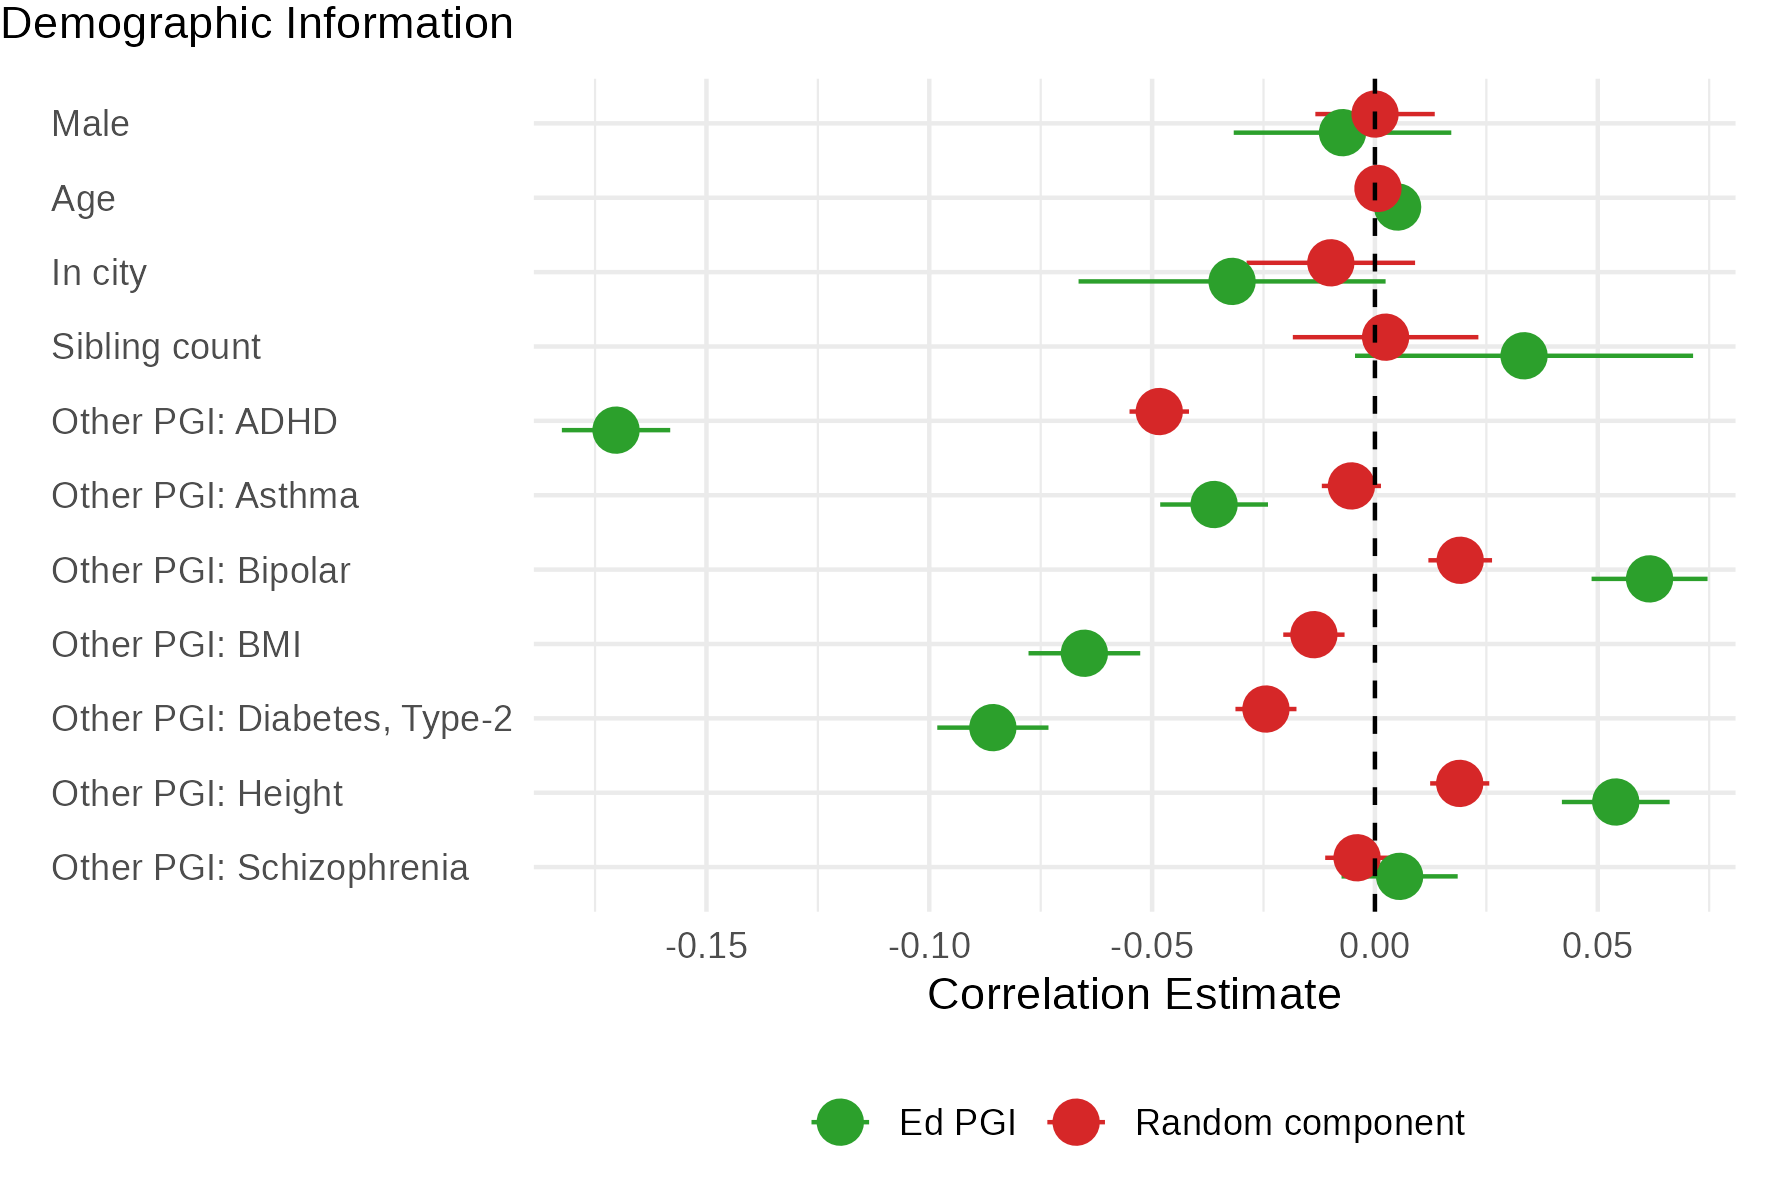
\includegraphics[width=0.85\textwidth]{
        sections/figures/demographic-correlates.png}
    \justify
    \footnotesize
    \textbf{Note}:
    Multivariate regression estimates for the linear model $Z_i = \vec \phi\,' \, \vec X_i + \eta_i$, where $\vec X_i$ is the vector demographic variables described by the labels on the $y$-axis.
    The dots are the point estimates, and bars are the 95\% confidence intervals.
    The random component refers to the Ed PGI after residualing out parental values,
\end{figure}

\subsection{Returns to Education by the MSLA Rise}
\label{appendix:MSLA}
The UK Biobank includes a total of 500,000 members of the British public, with a roughly even distribution of birth years over 1945--1965.
In 1972, the British government increased the Minimum School Leaving Age (MSLA) by one year, from age 15 to 16.
The change took effect at the start of the 1972-73 school year, and applied to those born on or after 1 September 1957.
The reform therefore induced extra school years for individuals born around date 1 September 1957.
British school children sit exams for the GCSE qualification at age 16, so the reform pushed a larger share of the UK Biobank cohorts to remain in school to 16 and to complete these qualifications.

The 1972 MSLA change has been previously used for labour market education returns \citep{oreopoulos2006estimating}, and (null) mortality effects of compulsory education \citep{clark2013effect}.
The UK Biobank population overlaps well with the birth date cutoff, and so has been used in a series of papers for estimating education returns in the UK Biobank, for health outcomes \citep{barcellos2023distributional,barcellos2025education,davies2018causal} and occupation imputed income \citep{barcellos2021effect}.

\begin{figure}[H]
    \centering
    \singlespacing
    \caption{Mean Effects of the MSLA Rise.}
    \begin{subfigure}[b]{0.495\textwidth}
        \centering
        %\caption{GCSE Completion Rate.}
        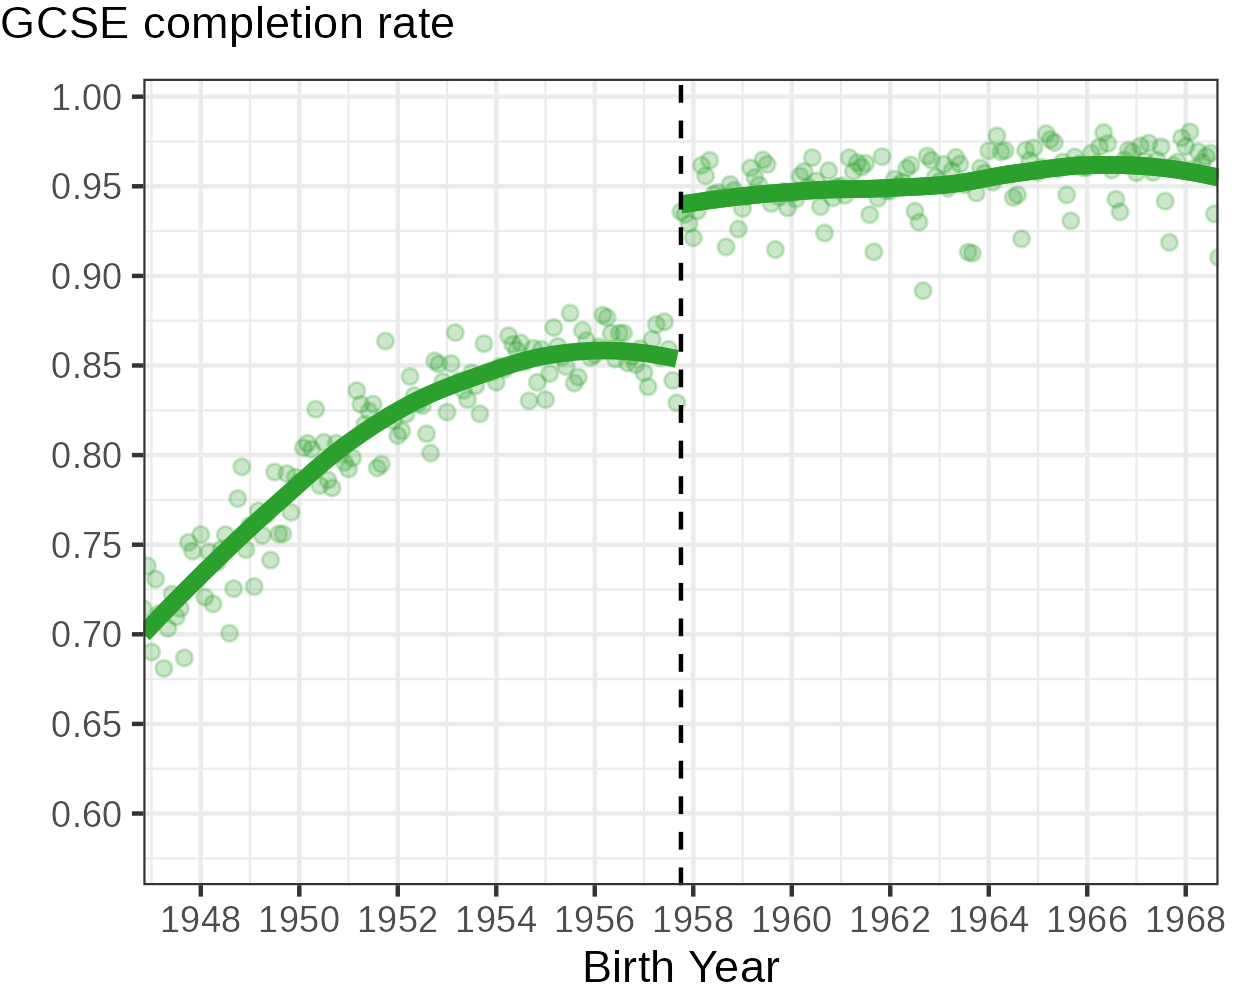
\includegraphics[width=\textwidth]{sections/figures/mlsa-gcses-nl.png}
    \end{subfigure}
    \begin{subfigure}[b]{0.495\textwidth}
        \centering
        %\caption{Mean Education years.}
        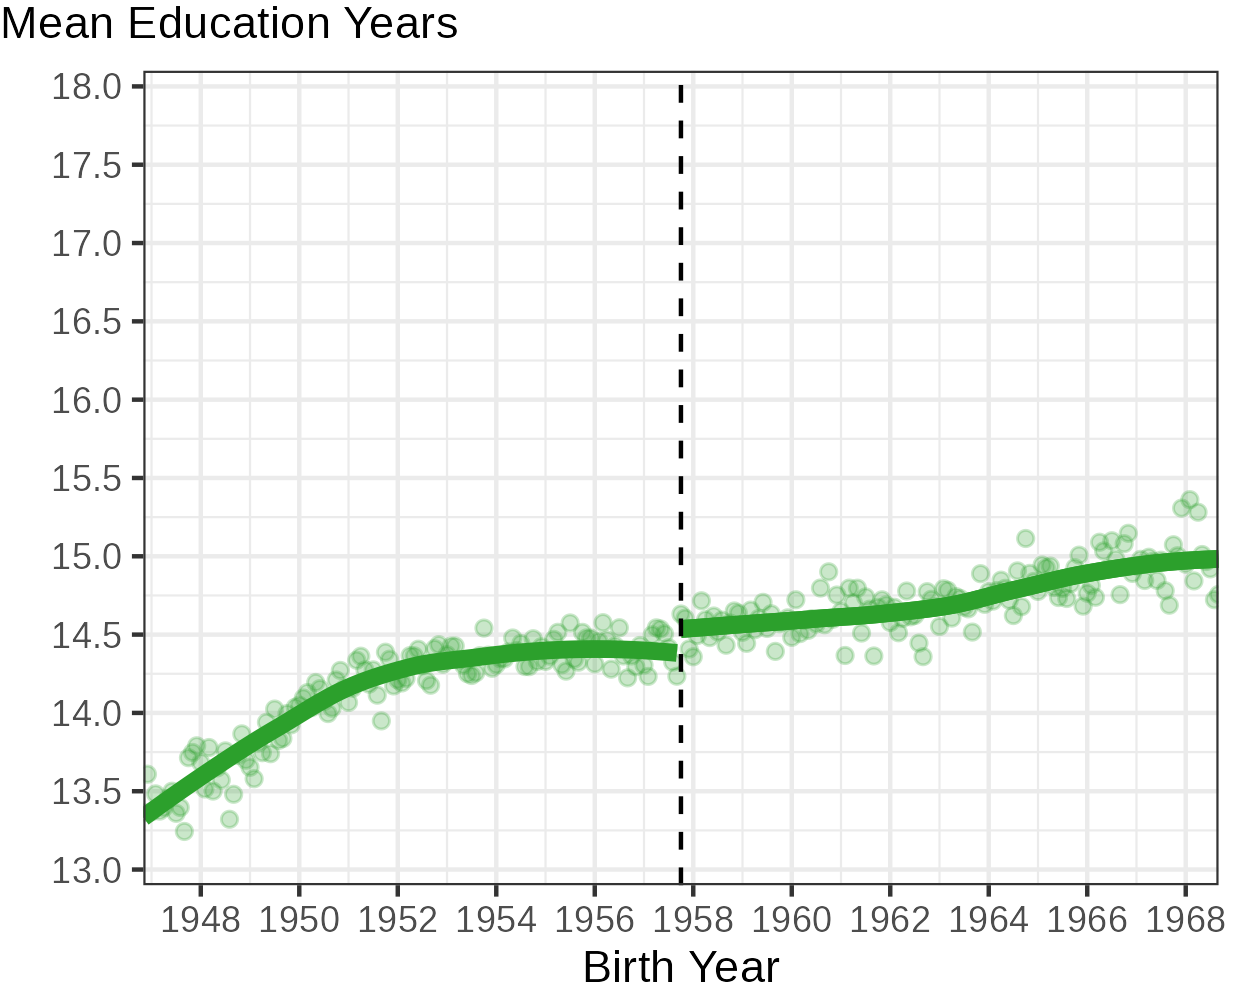
\includegraphics[width=\textwidth]{sections/figures/mlsa-edyears-nl.png}
    \end{subfigure}
    \begin{subfigure}[b]{0.495\textwidth}
        \centering
        %\caption{Rate of leaving school aged 16 or older.}
        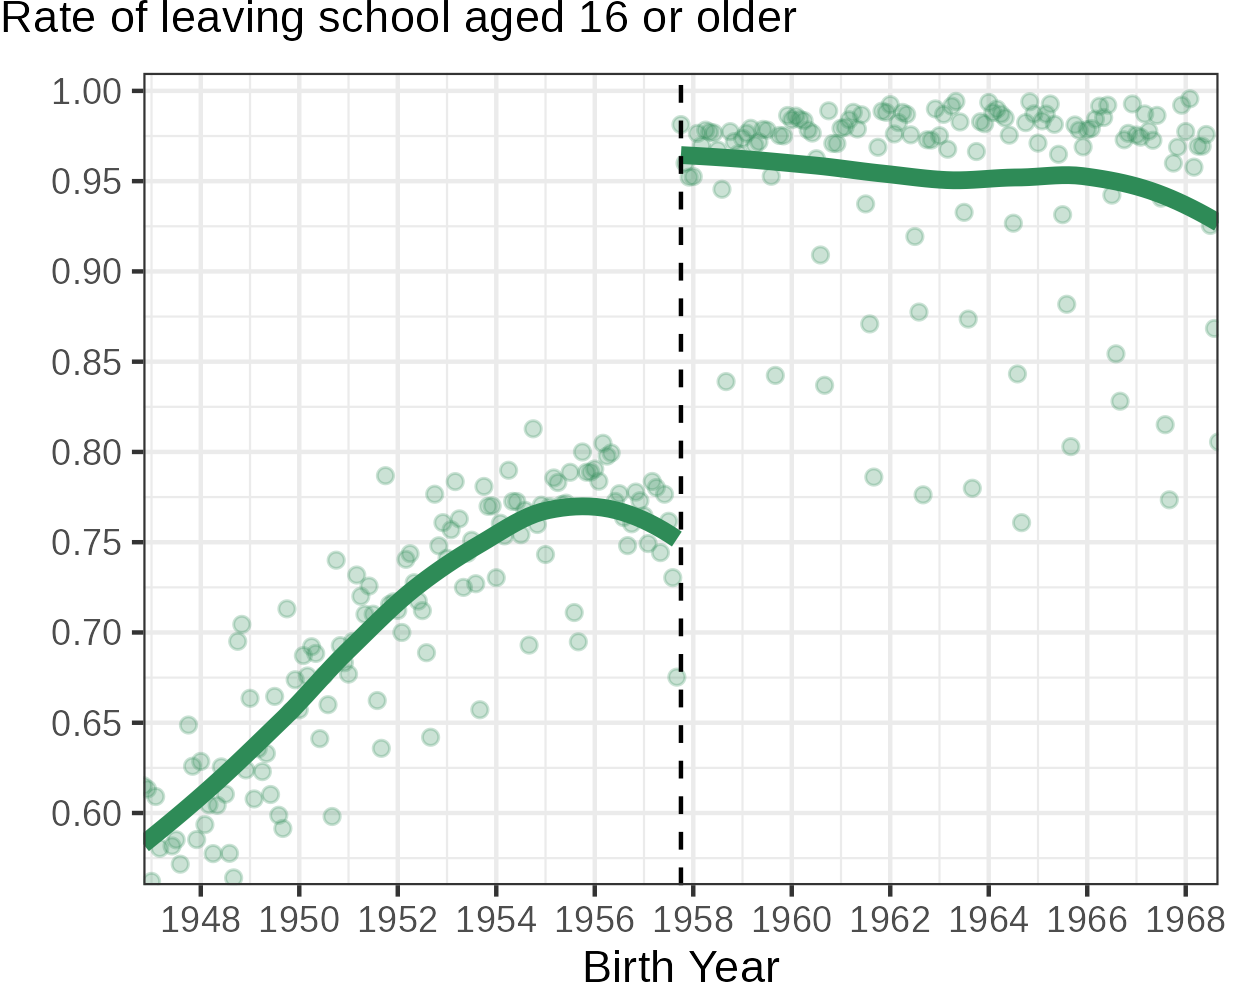
\includegraphics[width=\textwidth]{sections/figures/mlsa-edage16-nl.png}
    \end{subfigure}
    \begin{subfigure}[b]{0.495\textwidth}
        \centering
        %\caption{Mean age of leaving school.}
        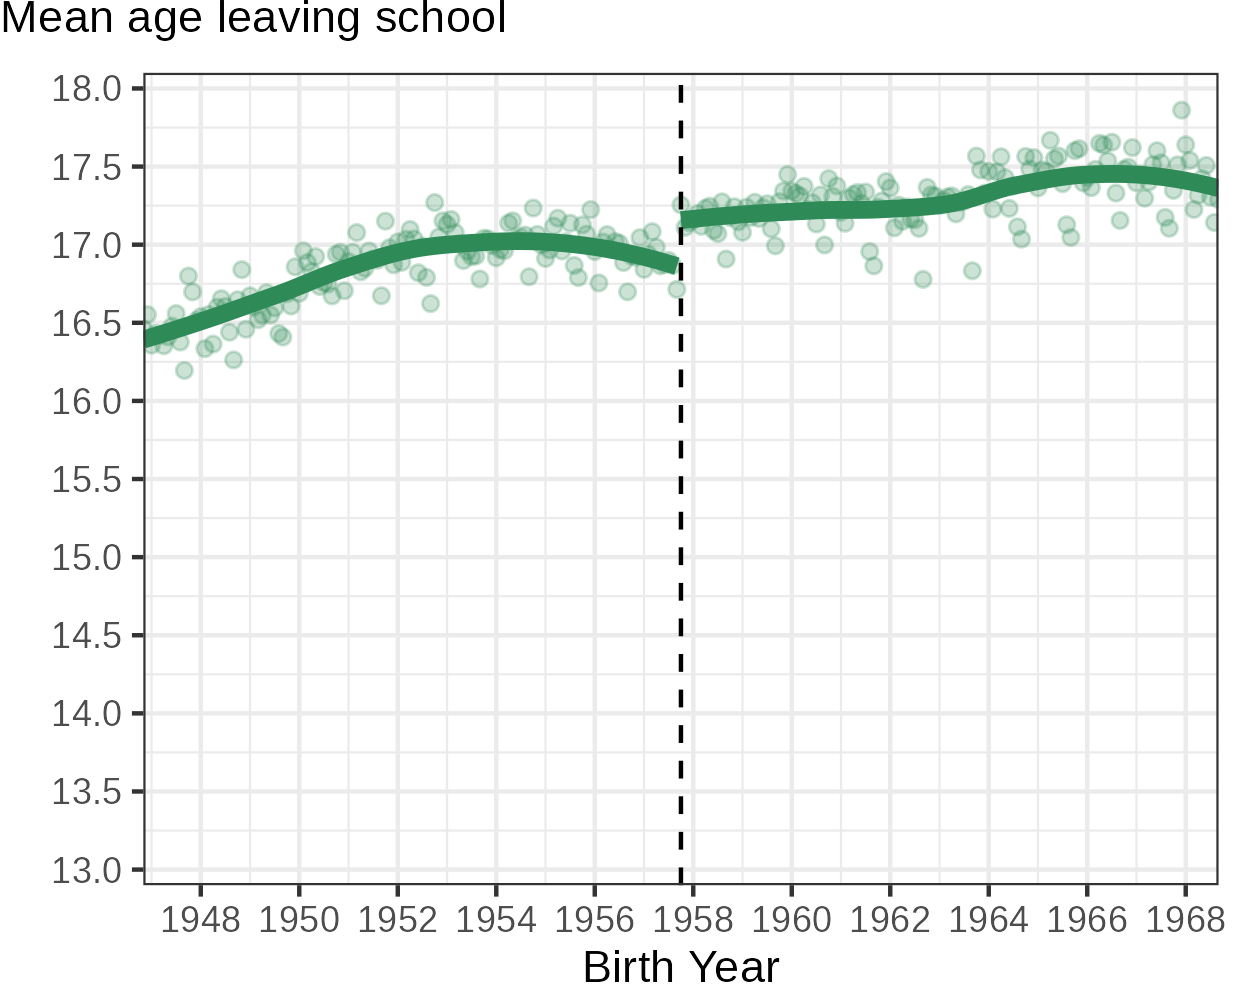
\includegraphics[width=\textwidth]{sections/figures/mlsa-agefinishededuc-nl.png}
    \end{subfigure}
    \begin{subfigure}[b]{0.495\textwidth}
        \centering
        %\caption{Occupation Hourly Wage.}
        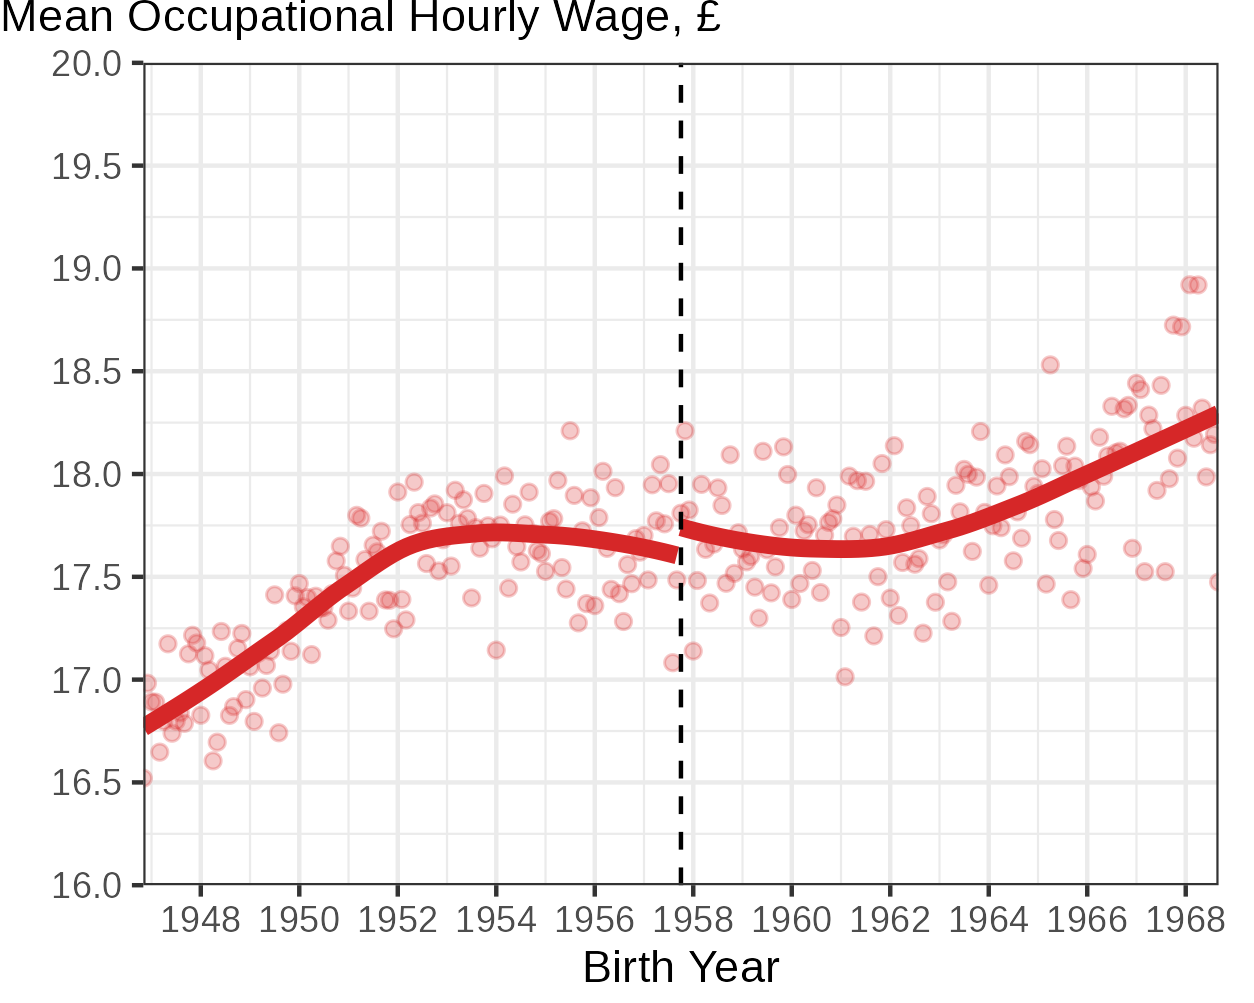
\includegraphics[width=\textwidth]{sections/figures/mlsa-wages-nl.png}
    \end{subfigure}
    \begin{subfigure}[b]{0.495\textwidth}
        \centering
        %\caption{Occupation Annual Income.}
        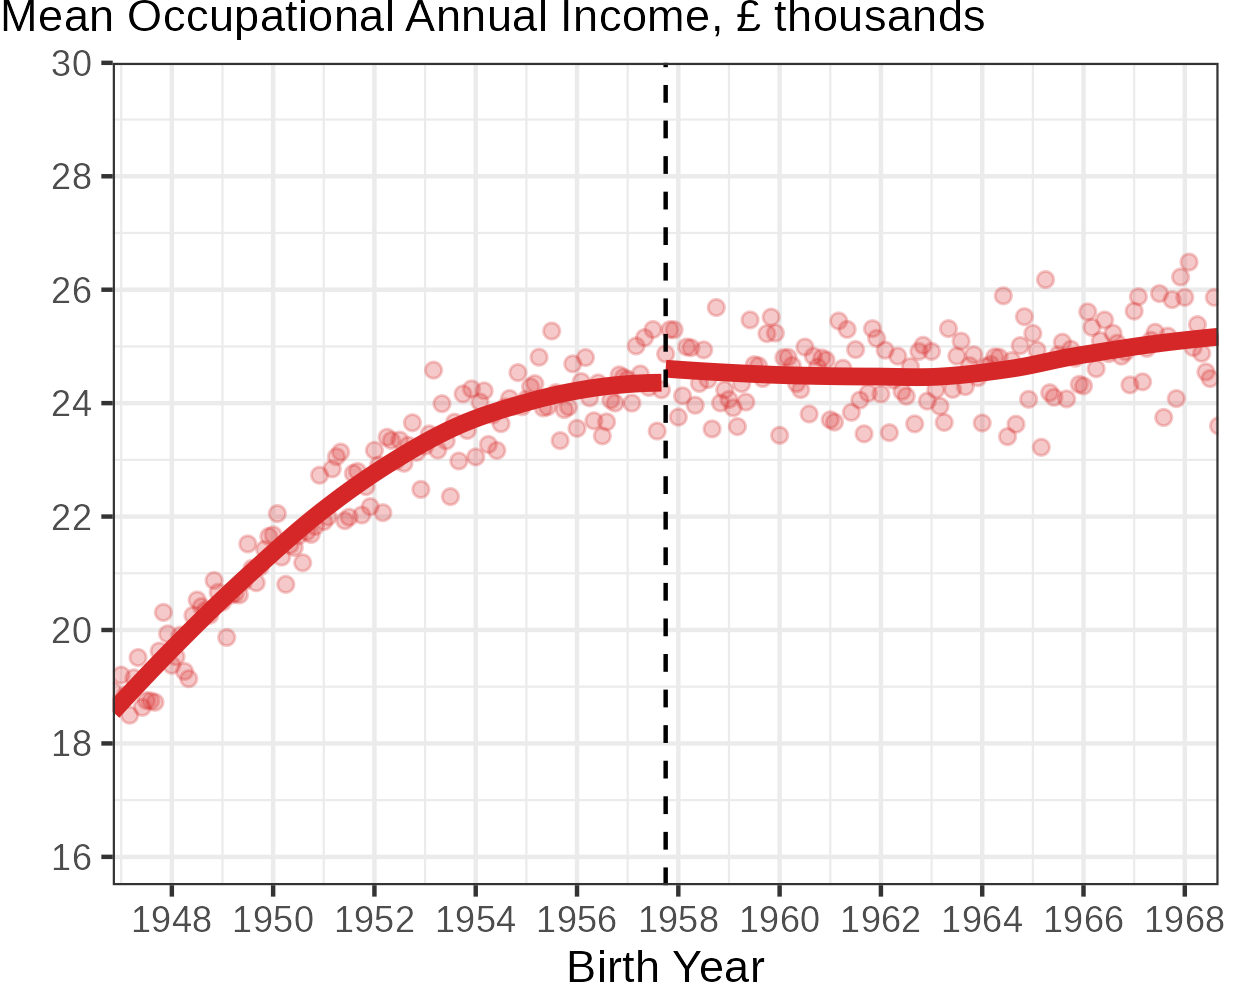
\includegraphics[width=\textwidth]{sections/figures/mlsa-income-nl.png}
    \end{subfigure}
    \label{fig:mlsa-nl}
    \vspace{-0.5cm}
    \justify
    \footnotesize
    \textbf{Note}:
    These figures show the effects of the 1972 MSLA rise on multiple outcomes, where individuals born after September 1957 (the dashed line) were legally compelled to stay in school until age 16, whereas before only until age 15.
    Each dot is the mean for UK Biobank respondents with non-missing education data born in that month-year, and the lines are local polynomials either side of September 1957.
\end{figure}

Birth month is the running variable in a fuzzy Regression Discontinuity Design (RDD), using the indicator for being born September 1957 and after as an instrument.
Because not all those eligible necessarily stayed beyond 15, the post-cutoff indicator instruments education variables, where mentioned.
I estimate the following RDD estimands, estimating the effect of the MSLA change on education variables --- represented by $D_i$.
\[ \lim_{v \to^- 1957.75} \Egiven{D_i}{V_i = v}, \;\;\;\;
    \lim_{v \to^+ 1957.75} \Egiven{D_i}{V_i = v} \]
where $V_i$ represents individual $i$'s birth year plus birth month divided by 12 (so that 1957.75 represents born in September 1957), and $\to^-$ refers to the limit from below, $\to^+$ above.
The goal is to identify the average compliance rate of the MSLA rise,
\[ \E{D_i(1) - D_i(0)}
    = \lim_{v \to^+ 1957.75} \Egiven{D_i}{V_i = v}
        - \lim_{v \to^- 1957.75} \Egiven{D_i}{V_i = v}. \]

The MSLA rise significantly increases education years, completing of age 16 secondary school qualifications (GCSEs) --- these are measured of education coded by qualifications, as used by \cite{okbay2022polygenic} in calculating the Ed PGI.
It had an even larger effect on age at leaving school, which is the basis of the education variables that \cite{barcellos2021effect} focuses on.
The mean of these variables by birth month are shown in \autoref{fig:mlsa-nl}.
Note that the economics literature has argued that null estimates for education returns in the MSLA design are a result of the MSLA rise inducing a low-quality margin of education \citep{clark2013effect}, so while age leaving education variables are more significant for this instrument they may not be economically relevant.

I also use the RDD design to measure changes in later labour market outcomes.
The UK Biobank asks questions of the sector people work in, giving high detail occupation codes (i.e., SOC codes).
Using this value, and other demographic details, I impute occupation coded income for the UK Biobank respondents using data from the British Annual Survey of Hours and Earnings.\footnote{
    Thanks to \cite{kweon2025associations} for sharing code on this imputation.
}
This gives occupation coded hourly income, and annual wage calculated from hours worked as outcome measures in the MSLA rise, affected by the MSLA rise
\[ \lim_{v \to^+ 1957.75} \Egiven{Y_i}{V_i = v}
    - \lim_{v \to^- 1957.75} \Egiven{Y_i}{V_i = v}. \]
The final panels of \autoref{fig:mlsa-nl} show these outcomes, and this reduced-form effect of the MSLA is not significantly different from zero.
\cite{barcellos2021effect} analyse this same RDD with UKB data.

\begin{table}[H]
    \singlespacing
    \small
    \centering
    \caption{Estimates of the MSLA Change Effects.}
    \centerline{
    \begin{tabular}{l c c c c c c c c}
        \\[-1.8ex]\hline \hline \\[-1.8ex]
        \textbf{Panel A: First-stage.}
        & \multicolumn{4}{c}{First-stage.}
            & \multicolumn{4}{c}{Reduced form.}\\
        \cmidrule(lr){2-5} \cmidrule(lr){6-9}
        %\multicolumn{1}{r}{Outcome:}
        Outcome:
        & \multicolumn{2}{c}{GCSE}       & \multicolumn{2}{c}{Education} & \multicolumn{2}{c}{Hourly} & \multicolumn{2}{c}{Annual} \\
        & \multicolumn{2}{c}{completion} & \multicolumn{2}{c}{years}     & \multicolumn{2}{c}{wage}   & \multicolumn{2}{c}{income} \\
        \cmidrule(lr){2-5} \cmidrule(lr){6-9}
        & (1) & (2) & (3) & (4) & (5) & (6) & (7) & (8) \\
        \\[-1.8ex]\hline \\[-1.8ex]
        % latex table generated in R 4.5.2 by xtable 1.8-4 package
% Wed Mar 11 18:38:49 2026
 MSLA Effect & 0.089 & 0.247 & 0.158 & 0.314 & 0.006 & 0.006 & 0.010 & 0.010 \\ 
    & (0.006) & (0.011) & (0.060) & (0.058) & (0.007) & (0.007) & (0.010) & (0.010) \\ 
  \\ $F$-statistics & 216 & 530 & 6.85 & 29.7 & 0.939 & 0.939 & 0.830 & 0.830 \\ 
  CCT bandwidth & 2.66 & 1.60 & 3.21 & 2.60 & 4.10 & 4.10 & 3.87 & 3.87 \\ 
  Bandwidth observations & 64,011 & 24,185 & 77,881 & 38,718 & 99,646 & 99,646 & 93,885 & 93,885 \\ 
  
        \\[-1.8ex]\hline \\[-1.8ex]
        \textbf{Panel B: Second-stage.}
            & \multicolumn{4}{c}{OLS.}
                & \multicolumn{4}{c}{MSLA IV.} \\
        \cmidrule(lr){2-5} \cmidrule(lr){6-9}
        & (1) & (2) & (3) & (4) & (5) & (6) & (7) & (8) \\
        \\[-1.8ex]\hline \\[-1.8ex]
        \multicolumn{8}{l}{Outcome: Log Occupation Hourly Wage} \\
        % latex table generated in R 4.5.2 by xtable 1.8-4 package
% Wed Mar 11 18:39:37 2026
 GCSE completion & 0.372 & 0.193 &   &   & 0.070 & 0.068 &   &   \\ 
    & (0.008) & (0.008) &   &   & (0.094) & (0.039) &   &   \\ 
  Education years &   &   & 0.061 & 0.034 &   &   & 0.044 & 0.057 \\ 
    &   &   & (0.000) & (0.002) &   &   & (0.047) & (0.029) \\ 
  \\ CCT bandwidth & 10.0 & 10.0 & 10.0 & 10.0 & 2.54 & 2.71 & 4.21 & 4.08 \\ 
  Bandwidth observations & 245,740 & 149,732 & 245,740 & 149,732 &  62,027 &  39,938 & 101,570 &  58,987 \\ 
  
        \\[-1.8ex]\hline \\[-1.8ex]
        \multicolumn{8}{l}{Outcome: Log Occupation Annual Income} \\
        % latex table generated in R 4.5.2 by xtable 1.8-4 package
% Wed Mar 11 18:40:28 2026
 GCSE completion & 0.392 & 0.188 &   &   & 0.100 & 0.046 &   &   \\ 
    & (0.015) & (0.009) &   &   & (0.151) & (0.065) &   &   \\ 
  Education years &   &   & 0.065 & 0.032 &   &   & 0.062 & 0.048 \\ 
    &   &   & (0.001) & (0.002) &   &   & (0.080) & (0.049) \\ 
  \\ CCT bandwidth & 10.0 & 10.0 & 10.0 & 10.0 & 2.61 & 2.86 & 3.84 & 4.16 \\ 
  Bandwidth observations & 245,740 & 149,732 & 245,740 & 149,732 &  64,011 &  42,307 &  93,885 &  60,155 \\ 
  \\[-1.8ex]\hline \\[-1.8ex] Qualification definition & Yes &   & Yes &   & Yes &   & Yes &   \\ 
  School age definition &   & Yes &   & Yes &   & Yes &   & Yes \\ 
  
        \\[-1.8ex]\hline \hline \\[-1.8ex]
    \end{tabular}
    }
    \vspace{-0.25cm}
    \label{tab:mlsa-iv}
    \justify
    \footnotesize
    \textbf{Note:}
    These point estimates are calculated among all UK Biobank participants born within a bandwidth of the MSLA rise cutoff (not just the sibling subsample).
    The odd columns use a definition of education attainment (age 16 schooling) based on reported education qualifications; even columns report based on school leaving age.
    The Panel B OLS results show estimates of an OLS specification for the correlation between education and wages/income with local polynomial trends each side of 1957.75 birthdate, attempting to mimic an RD set-up with a hard-coded bandwidth of 10 years for comparison.
\end{table}

I estimate this RDD equation with triangular kernel weights (weighting closer to the cutoff), an optimal bandwidth \citep{calonico2014robust,calonico2015rdrobust}, and non-parametric controls on either side of the cutoff \citep{gelman2019high}.
These estimates are collected in \autoref{tab:mlsa-iv}.

\begin{figure}[H]
    \centering
    \singlespacing
    \caption{Fuzzy RDD Estimates, Sensitivity to Bandwidth Choice.}
    \begin{subfigure}[b]{0.495\textwidth}
        \centering
        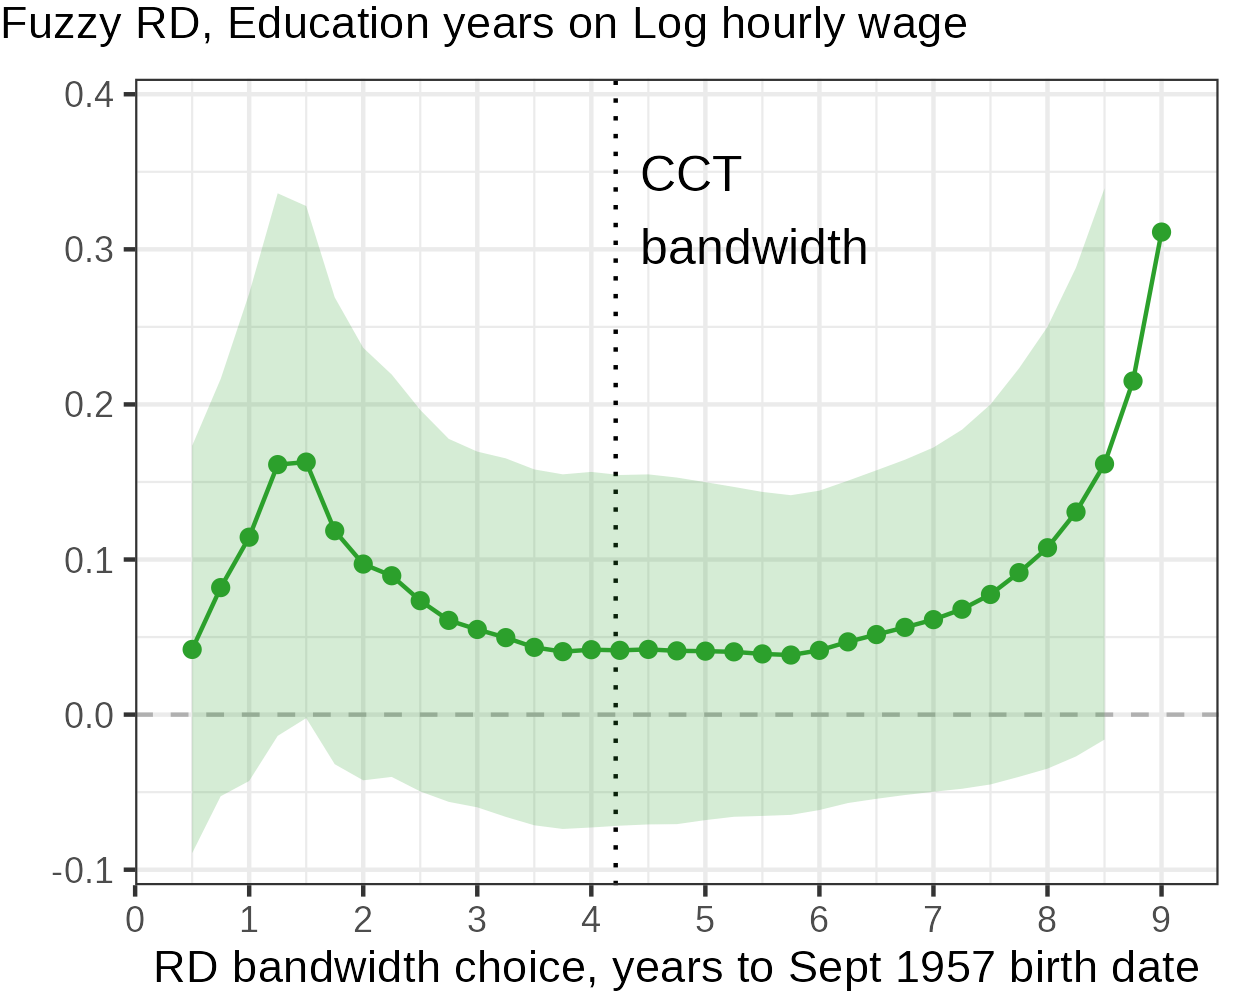
\includegraphics[width=\textwidth]{sections/figures/mlsa-edyears-bw.png}
    \end{subfigure}
    \begin{subfigure}[b]{0.495\textwidth}
        \centering
        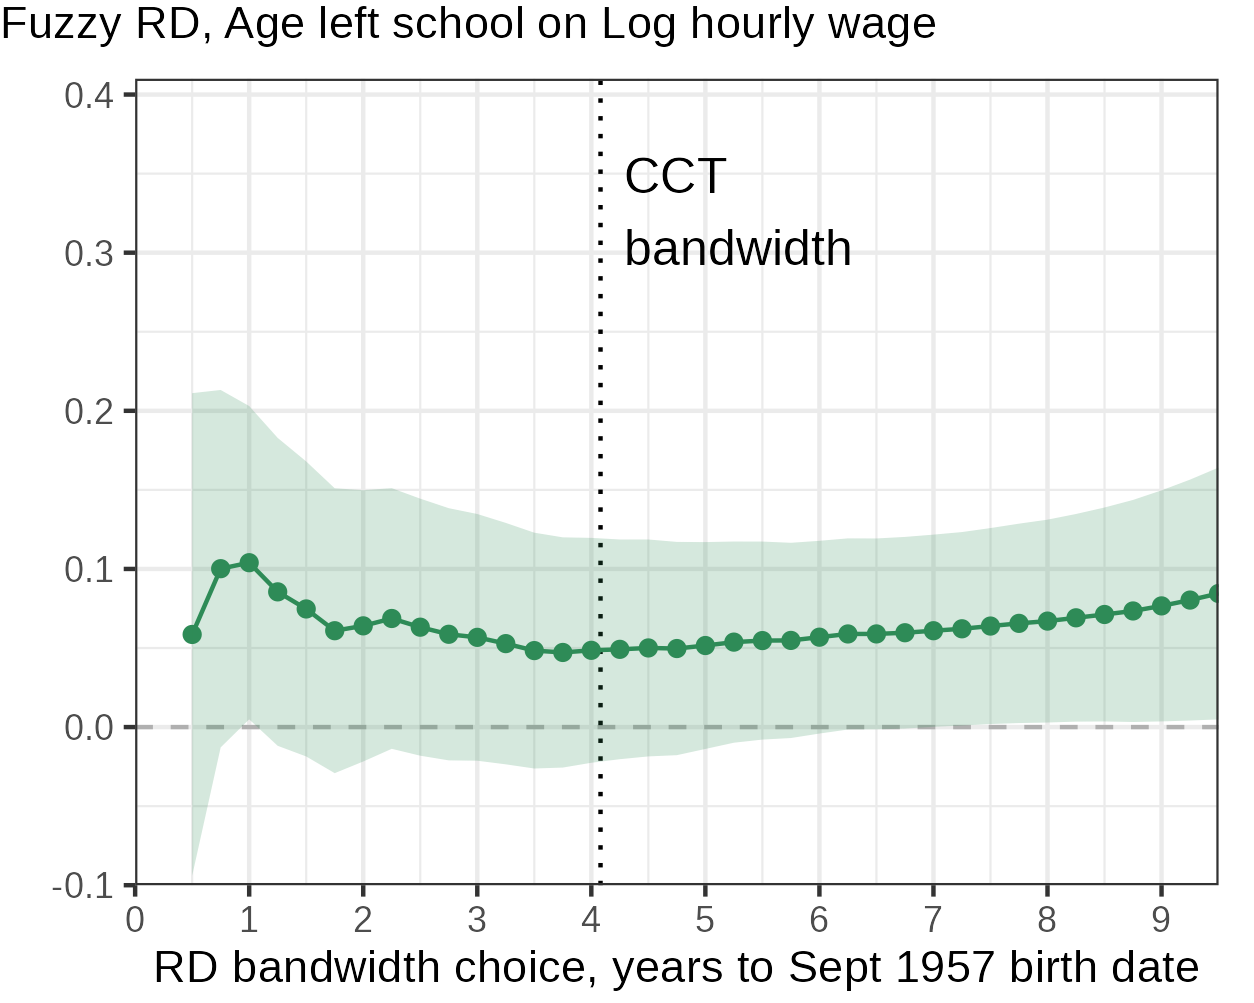
\includegraphics[width=\textwidth]{sections/figures/mlsa-edage-bw.png}
    \end{subfigure}
    \label{fig:mlsa-bw}
    \vspace{-0.5cm}
    \justify
    \footnotesize
    \textbf{Note}:
    These figures show the sensitivity of fuzzy RD estimates using the MSLA discontinuity as an IV for education years (qualification measure) or age leaving school, using a different bandwidth choice for each.
    The shaded regions are the 95\% confidence interval.
    The dotted line with CCT refers to the \cite{calonico2014robust} optimal bandwidth choice, calculated using \textit{rdrobust} in \textit{R} \citep{calonico2015rdrobust}.
\end{figure}

The MSLA rise increased years of education, as measured in both qualification definitions and school leaving age definition.
However, the outcome of occupation coded wages and annual income are not strong; correspondingly, the IV estimates using the MSLA rise for education returns are not distinguishable from zero.
This holds true for a range of bandwidth choices, shown in \autoref{fig:mlsa-bw}.

\subsection{Instrumental Variables Connection}
\label{appendix:iv}
The CM analysis in this paper is conceptually similar to an instrumental variables analysis; the main difference is that it does not assume the exclusion restriction, and instead attempts to model and estimate this direct effect.
One might consider using the Ed PGI as an instrument for education years, interpreting the reduced-form effect of the Ed PGI on earnings only through its first-stage effect on education. 
This is the logic of Mendelian Randomisation (MR), where genetic variants are used as instruments for health conditions, and any direct effect of the genetic index on the outcome is treated as a violation of the exclusion restriction.

\cite{widding2026}, for example, uses the Ed PGI as an instrument for education in an MR design; this approach is not well suited to the present question as it assumes the direct effects are exactly zero for every individual, giving estimates for returns to education contaminated by plausibly non-zero direct effects.
The CM approach instead estimates both the direct genetic effect and the indirect education effect.

There is a literature for modelling such exclusion violations in economics \citep{conley2012plausibly,kolesar2015}, and in genetic settings using alternative assumptions tailored to MR \citep{bowden2015mendelian,spiller2019detecting}.
These alternative approaches require structure on how invalid instruments violate exclusion; the most common adjustment for genetic settings, MR-egger \citep{bowden2015mendelian}, relies on the direct genetic effects being uncorrelated with instrument strength, paralleling the invalid instruments assumption in the econometrics literature \citep{kolesar2015}. 
This is difficult to justify in the present setting, where the SNPs that most strongly predict education could have correspondingly larger direct effects on earnings through cognitive skills, non-cognitive traits, health, field of study, occupational sorting, or other labour-market relevant channels.

\subsection{Returns to Education Literature}
\begin{table}[!htbp]
    \small
    \singlespacing
    \centering
    \vskip-0.75cm
    \caption{Returns to Education, British Estimates from the Literature.}
    \centerline{
    \begin{tabular}{c c c p{12.75cm}}
        \toprule
        OLS & IV   & Year & Reference \\ \midrule
        29.2 & 5.7 &  2010 & Dickson, M. and Smith, S., 2011. What determines the return to education: an extra year or a hurdle cleared?. Economics of education review, 30(6), pp.1167-1176. \\
        12.2 & 6.6 &  2009 & Devereux, P.J. and Fan, W., 2011. Earnings returns to the British education expansion. Economics of Education Review, 30(6), pp.1153-1166. \\
        9.6 & 5.3 &   2009 & Devereux, P.J. and Fan, W., 2011. Earnings returns to the British education expansion. Economics of Education Review, 30(6), pp.1153-1166. \\
        9.5 & 6.9 &   2006 & Grenet, J. 2013. Is it enough to increase compulsory education to raise earnings? Evidence from French and British compulsory schooling laws. Scandinavian Journal of Economics 115: 176-210. \\
        7.8 & 6.2 &   2009 & Devereux, P.J. and Fan, W., 2011. Earnings returns to the British education expansion. Economics of Education Review, 30(6), pp.1153-1166. \\
        6.0 & 4.4 &   1999 & Blanchflower, D. and Elias, P., 1999. Ability, schooling and earnings: Are twins different?. Unpublished manuscript, Warwick University. \\
        6.9 & 6.6 &   2009 & Devereux, P.J. and Fan, W., 2011. Earnings returns to the British education expansion. Economics of Education Review, 30(6), pp.1153-1166. \\
        7.0 & 7.0 &   2001 & Devereux, P.J. and R.A. Hart. 2010. Forced to be Rich? Returns to Compulsory Schooling in Britain. Economic Journal 120(549): 1345-64. \\
        7.3 & 7.7 &   1999 & Bonjour, D., Cherkas, L.F., Haskel, J.E., Hawkes, D.D. and Spector, T.D., 2003. Returns to education: Evidence from UK twins. American Economic Review, 93(5), pp.1799-1812. \\
        4.8 & 5.5 &   1991 & Dearden, Lorraine. 1999. Qualifications and earnings in Britain: how reliable are conventional OLS estimates of the returns to education? IFS Working Papers W99/07, Institute for Fiscal Studies. \\
        4.8 & 5.5 &   1981 & Dearden, L. (1998), ``Ability, Families, Education and Earnings in Britain,'' Institute for Fiscal Studies Working Paper No. W98/14. \\
        0.0 & 1.2 &   1947 & Chib, Siddhartha, and Liana Jacobi. 2016. “Bayesian Fuzzy Regression Discontinuity Analysis and Returns to Compulsory Schooling.” Journal of Applied Econometrics 31: 1026-1047. \\
        5.0 & 9.9 &   1970s & Harmon, C. and Walker, I. (2000), ``Returns to the Quantity and Quality of Education: Evidence for Men in England and Wales,'' Economica, 67: 19-35. \\
        4.6 & 10.2 &  1972 & Dickson, Matt. 2013. “The Causal Effect of Education on Wages Revisited.” Oxford Bulletin of Economics and Statistics 75 (4): 477-498. \\
        7.8 & 14.7 &  1947 & Oreopoulos, P. 2006. Estimating Average and Local Average Treatment Effects of Education when Compulsory Schooling Laws Really Matter American Economic Review96(1) 152-175 \\
        4.9 & 14.0 &  1992 & Harmon, C. and Walker, I. (1999), ``The Marginal and Average Return to Schooling in the UK,'' European Economic Review, 43(4-6), pp.879-887. \\
        6.1 & 15.3 &  1947 & Harmon, C. and I. Walker. 1995. Estimates of the economic return to schooling for the United Kingdom. American Economic Review 85: 1278-86. \\
        \bottomrule
    \end{tabular}}
    \label{tab:uk-meta}
    \justify
    \footnotesize
    \textbf{Note:}
    This table shows the education returns estimates on later-life labour market earnings in the economics literature, using an IV to causally estimate the effect of a year of education.
    Literature review kindly provided by \cite{patrinos2025causal}.
\end{table}
